% 第 4 周交付物:基线模型验证与性能基准报告(中文版) —— 编译方式:XeLaTeX
\documentclass[11pt]{ctexart}
\usepackage[a4paper, margin=2.4cm]{geometry}
\usepackage{amsmath}
\usepackage{booktabs}
\usepackage{graphicx}
\usepackage[hidelinks]{hyperref}
\usepackage{enumitem}
\setlist{nosep}

\title{\textbf{基线模型验证与性能基准报告}\\
\large Advanced Chooser Option Pricing Model --- 第 4 周交付物}
\author{佟铸城 (Zhucheng Tong)}
\date{2026 年 8 月}

\begin{document}
\maketitle

\section{评估设计}
经导师确认以蒙特卡洛替代 CME 成交价后,基线评估分三层,每层回答一个不同的问题:
\begin{enumerate}
  \item \textbf{实现正确性}(MC $\leftrightarrow$ 闭式解):代码算得对不对;
  \item \textbf{假设失效}(回望校准 $\leftrightarrow$ 事后真值):BSM 常数波动率假设在真实数据上的代价有多大、集中在什么状态——本层是核心,其误差水平即第 5--6 周 ML 要打败的\textbf{基准线};
  \item \textbf{选择规则代价}(真实利率状态复检):第 3 周发现的"论文 moneyness 规则代价随利率放大"在真实数据日期上的验证。
\end{enumerate}

评估口径:每个交易日以当日现价为行权价(ATM)、$t_1=0.5$、$T_2=1$ 年发行一份新 chooser;
$r$ 取当日 1 年期国债收益率,$q$ 取 TTM 股息率;\textbf{事后真值(oracle)价格}用该期权存续一年内\textbf{实际实现}的波动率定价。
样本 1310 个交易日(2019-10-17 至 2024-12-31),事后真值窗口用到 2025-12 的数据(自动化管道已采集)。

\section{第一层:实现正确性(MC 收敛的 MAE/RMSE)}
论文参数下闭式解 \$29.1299;各路径数下 30 次独立种子的 MC 估计误差:

\begin{center}
\begin{tabular}{rrrr}
\toprule
\textbf{路径数} & \textbf{MAE} & \textbf{RMSE} & \textbf{MAE 占价格} \\
\midrule
1{,}000 & 0.534 & 0.681 & 1.83\% \\
10{,}000 & 0.124 & 0.158 & 0.43\% \\
100{,}000 & 0.051 & 0.061 & 0.18\% \\
\bottomrule
\end{tabular}
\end{center}

误差按 $1/\sqrt{n}$ 收敛(路径数 $\times100$,误差 $\div10$),实现正确性确立。

\section{第二层:BSM 常数波动率假设的代价(核心基准)}

\subsection{总体误差}
四种回望校准与事后真值的逐日定价误差(1310 天):

\begin{center}
\begin{tabular}{lrrr}
\toprule
\textbf{$\sigma$ 估计器} & \textbf{MAE (\$)} & \textbf{RMSE (\$)} & \textbf{相对 MAE} \\
\midrule
21 日已实现 & 9.80 & 14.40 & 36.1\% \\
63 日已实现 & 9.76 & 13.37 & 37.4\% \\
252 日已实现 & 10.37 & 13.61 & 41.7\% \\
\textbf{EWMA($\lambda$=0.94)} & \textbf{9.44} & \textbf{13.52} & \textbf{35.3\%} \\
\bottomrule
\end{tabular}
\end{center}

最好的回望校准(EWMA)相对误差仍达 \textbf{35\%}——这就是常数波动率假设在 1 年期 ATM chooser 上的真实代价,也是 ML 模型的\textbf{起跑线}(基准表已存 \texttt{docs/week4/baseline\_metrics.csv})。

\begin{figure}[h!]
\centering
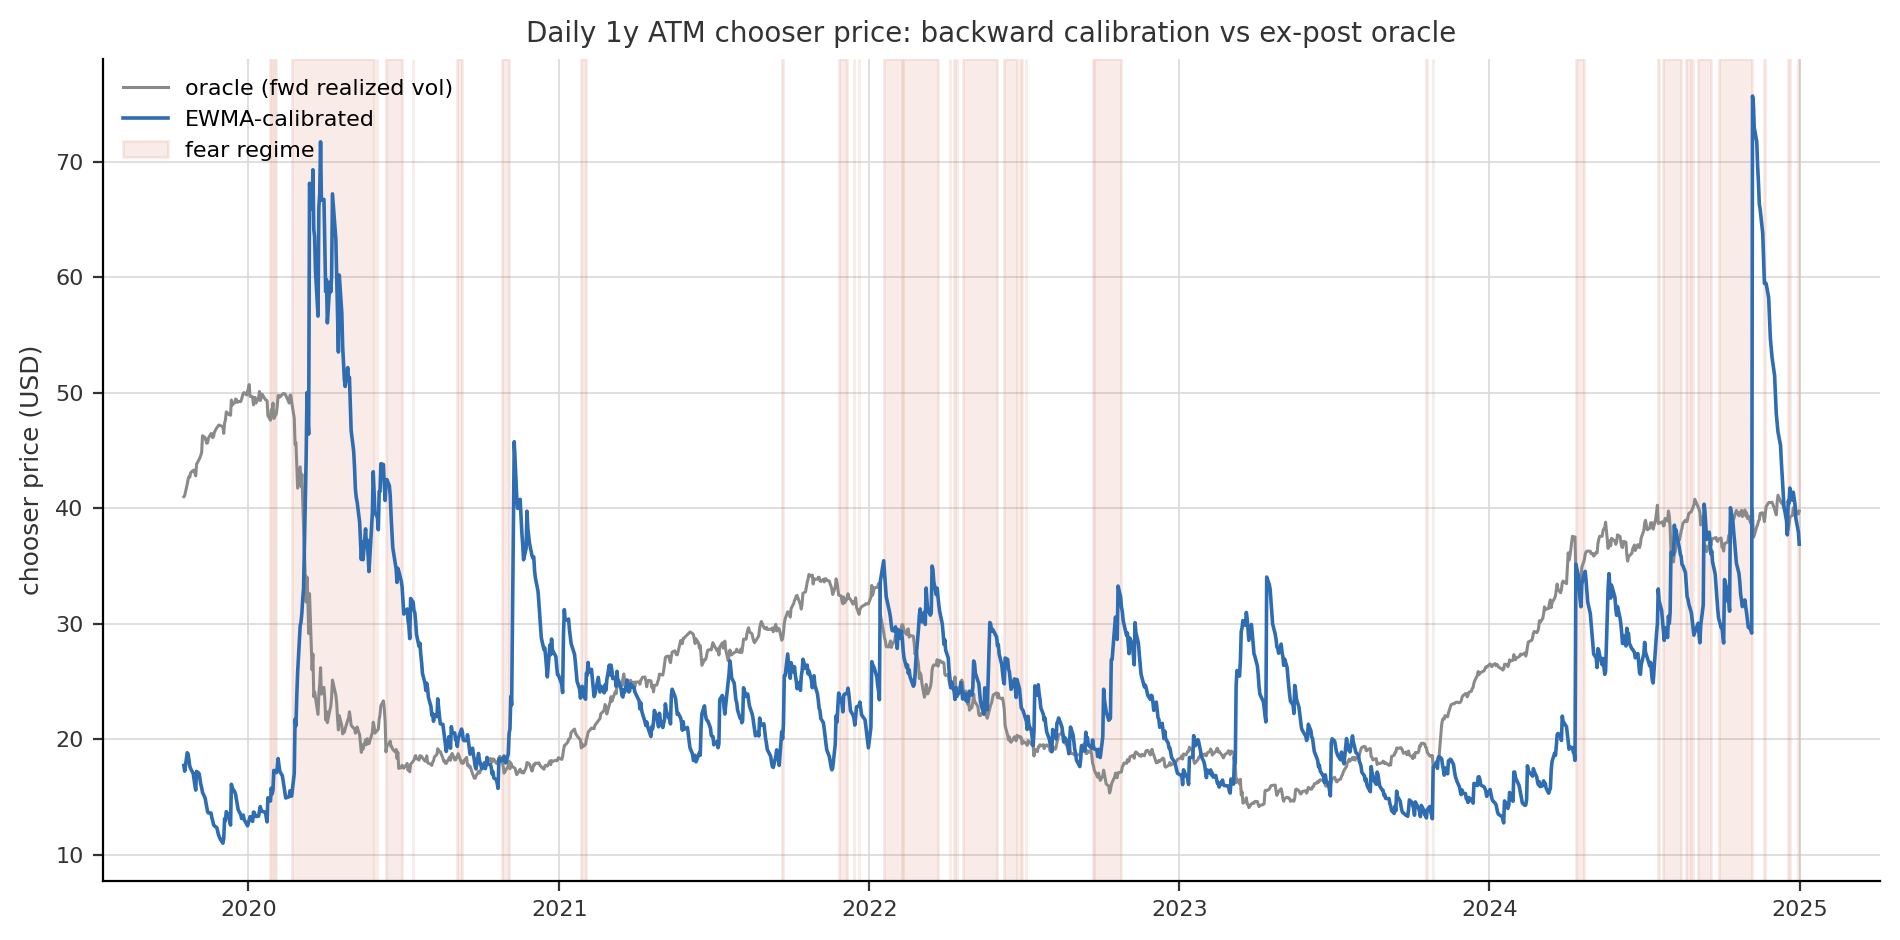
\includegraphics[width=0.96\textwidth]{figures/rolling_price.png}
\caption{逐日定价:EWMA 回望校准(蓝) vs 事后真值(灰);阴影为恐慌状态。2020 年初灰线先行抬升而蓝线浑然不觉——BSM 在危机前系统性低估、危机后系统性高估}
\end{figure}

\subsection{失效模式:取决于估计器的记忆长度}
按恐慌状态(第 2 周的 \texttt{fear\_regime})分组:

\begin{center}
\begin{tabular}{lrrl}
\toprule
\textbf{$\sigma$ 估计器} & \textbf{平静期 MAE} & \textbf{恐慌期 MAE} & \textbf{失效场景} \\
\midrule
21 日已实现 & 9.31 & 11.38 & 恐慌期(追高) \\
EWMA & 9.01 & 10.83 & 恐慌期(追高) \\
252 日已实现 & \textbf{10.94} & 8.55 & \textbf{危机后的平静期(拖尾)} \\
\bottomrule
\end{tabular}
\end{center}

两类失效模式方向相反:\textbf{快估计器}(21日/EWMA)在恐慌期跟随波动率飙升,而期权存续期内实际波动率会均值回复,导致\textbf{危机中高估};\textbf{慢估计器}(252日)则在危机结束后整整一年内窗口里仍拖着危机数据,导致\textbf{危机后的平静期持续高估}(2021 年:252 日校准 MAE \$10.34 vs 21 日校准 \$6.13)。\textbf{没有任何单一回望窗口在所有状态下占优}——这正是第 5 周让 ML 有条件地组合各窗口信息(含前瞻性 VIX 特征)的直接动机。

\begin{figure}[h!]
\centering
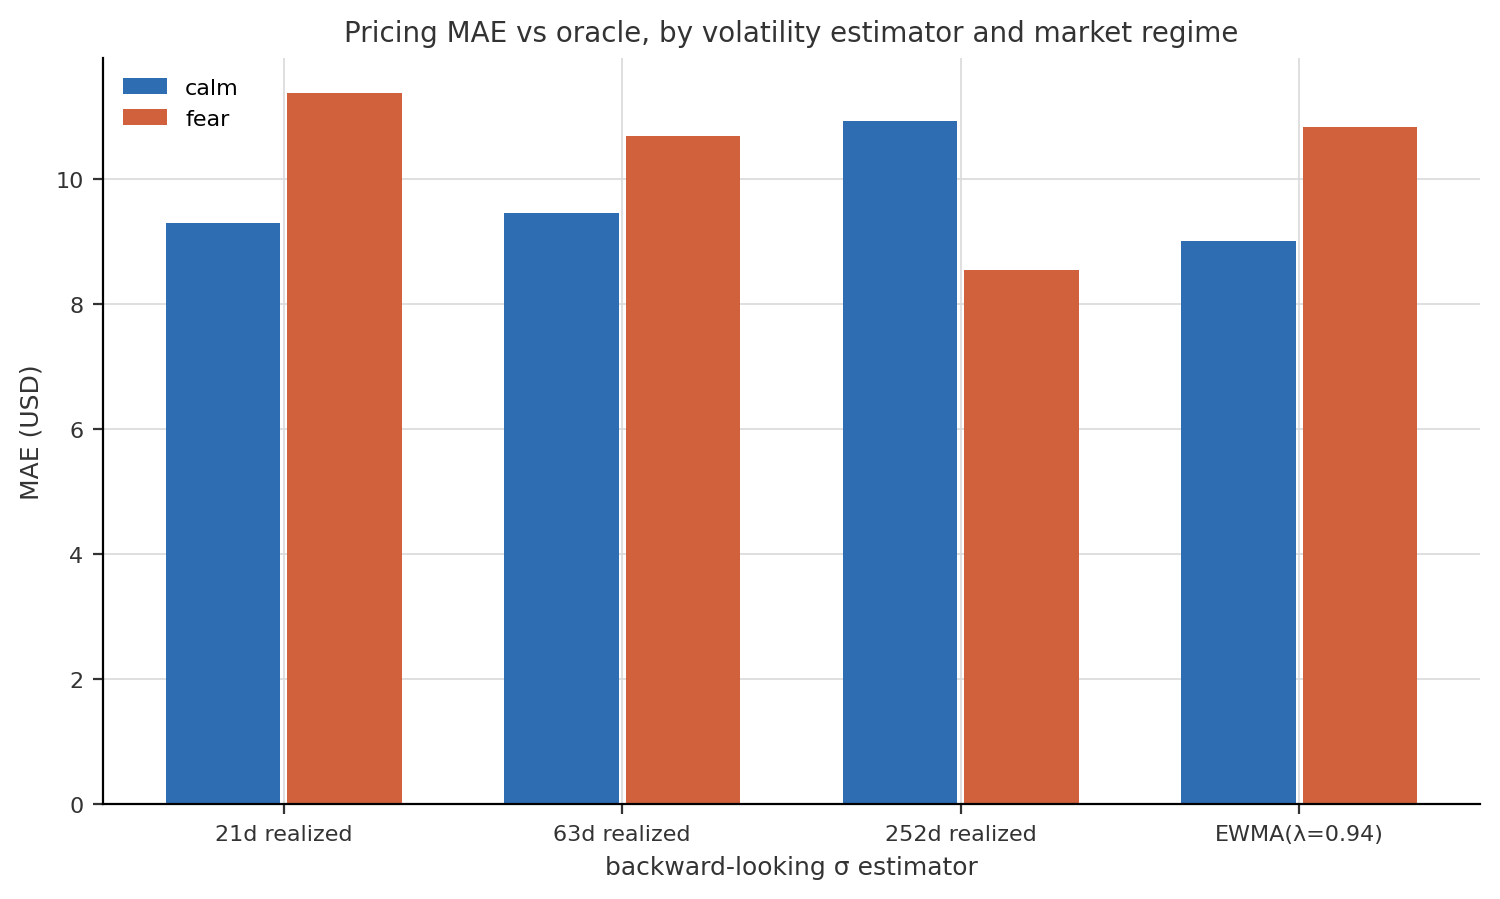
\includegraphics[width=0.62\textwidth]{figures/mae_by_regime.png}
\caption{分状态 MAE:快估计器恐慌期更差,252 日估计器平静期更差}
\end{figure}

\subsection{按年份的误差与两个诚实的说明}
\begin{center}
\begin{tabular}{lrrrrrr}
\toprule
& \textbf{2019(尾)} & \textbf{2020} & \textbf{2021} & \textbf{2022} & \textbf{2023} & \textbf{2024} \\
\midrule
EWMA 校准 MAE (\$) & 31.78 & 17.42 & 6.48 & 3.86 & 5.36 & 9.40 \\
\bottomrule
\end{tabular}
\end{center}

\begin{enumerate}
  \item \textbf{2019 年尾段误差(\$31.8)不可归咎于估计器}:这些日期的存续窗口覆盖 COVID 崩盘,属于任何回望方法都不可预见的突发跳变。它设定了一个现实的期望:ML 能改善的是\textbf{可预测的波动率动态}(聚集、均值回复、状态切换),而非黑天鹅本身;
  \item \textbf{EWMA 对单日跳变会过度反应}:2024-11 大选日 JPM 单日 $+11.5\%$ 使 EWMA 波动率瞬时翻倍、定价短暂冲高(见图 1 尾部尖峰),数日后消退——单日跳变与持续性波动状态的区分,同样是 ML 特征(如 VIX 动量 vs 水平)可以着力的点。
\end{enumerate}

\section{第三层:选择规则代价的真实数据复检}
\begin{center}
\begin{tabular}{lrrr}
\toprule
\textbf{真实日期} & \textbf{$r$(1年期)} & \textbf{规则代价 (\$)} & \textbf{基点} \\
\midrule
2021-06-30(低利率) & 0.07\% & 0.029 & 14.4 bp \\
2023-10-02(高利率) & 5.49\% & 0.047 & 32.2 bp \\
\bottomrule
\end{tabular}
\end{center}
第 3 周的结论在真实数据上成立:利率从 0.07\% 升至 5.49\%,论文 moneyness 规则的代价约 \textbf{2.2 倍}放大。本项目全程采用理性规则($\max(C,P)$)。

\section{扩展指标体系与加权综合评分(v2,应导师要求新增)}

\subsection{八项指标}
在 MAE/RMSE 之外扩充六项,按``一个定价模型什么情况下不可用''的逻辑分五族:

\begin{center}
\small
\begin{tabular}{llp{7.2cm}}
\toprule
\textbf{指标族} & \textbf{指标} & \textbf{衡量什么} \\
\midrule
平均精度 & MAE、RMSE、MedAE & 常规误差水平;MedAE(中位绝对误差)对极端日不敏感,与 MAE 的差距反映误差分布的偏斜 \\
方向偏差 & Bias(带符号均值误差) & 系统性高估/低估——对做市报价而言,方向性偏差比对称噪声更危险 \\
尾部/稳健 & P95AE、RegimeWorstMAE & 95 分位绝对误差(最差 5\% 交易日);两状态(平静/恐慌)中较差一侧的 MAE——模型不能靠牺牲某一状态换取平均好看 \\
解释力 & $R^2$(对 oracle 价格水平) & 相对``永远预测均值''的改进 \\
可用率 & Hit10(相对误差 $<10\%$ 的天数占比) & 日粒度的``报价可用''比例 \\
\bottomrule
\end{tabular}
\end{center}

\subsection{加权综合公式}
每项指标先统一为``越小越好''($1-R^2$、$1-\text{Hit10}$、$|\text{Bias}|$),再除以\textbf{参照模型}(EWMA 基线)的对应值得到比值(参照模型恒为 1),最后加权求和:
\[
\text{Composite}(m) \;=\; \sum_i w_i \cdot \frac{\text{metric}_i(m)}{\text{metric}_i(\text{EWMA})},
\qquad \sum_i w_i = 1 .
\]
权重:MAE 0.20、RMSE 0.10、MedAE 0.05(平均精度合计 0.35);P95AE 0.15、RegimeWorstMAE 0.15(尾部/稳健合计 0.30);$|$Bias$|$ 0.10;$1-R^2$ 0.10;$1-$Hit10 0.15。\textbf{设计理由}:稳健性族与平均精度族权重相当——定价模型靠``平均正确、危机崩溃''是不可接受的;比值化使综合分有直接读法:\textbf{Composite $<1$ 即优于 EWMA 基线},且第 5--6 周新增 ML 模型时无需重新归一。

\subsection{基线结果与两个诚实的结论}
\begin{center}
\small
\begin{tabular}{lrrrrrrrrr}
\toprule
& \textbf{MAE} & \textbf{RMSE} & \textbf{MedAE} & \textbf{Bias} & \textbf{P95} & \textbf{Worst} & \textbf{$R^2$} & \textbf{Hit10} & \textbf{综合分} \\
\midrule
21 日已实现 & 9.80 & 14.40 & 5.78 & $-1.78$ & 34.71 & 11.38 & $-1.39$ & 24.0\% & 1.067 \\
63 日已实现 & 9.76 & 13.37 & 7.31 & $-0.99$ & 33.52 & 10.70 & $-1.06$ & 16.1\% & 0.994 \\
252 日已实现 & 10.37 & 13.60 & 8.17 & $+0.70$ & \textbf{30.73} & 10.94 & $-1.13$ & 19.2\% & \textbf{0.982} \\
EWMA($\lambda$=0.94) & \textbf{9.44} & 13.52 & 6.32 & $-1.29$ & 34.39 & 10.83 & $-1.11$ & 22.4\% & 1.000 \\
\bottomrule
\end{tabular}
\end{center}

\begin{enumerate}
  \item \textbf{回望基线之间实质打平}:前三名综合分差距 $<2\%$,且排名对权重方案敏感(主权重与稳健导向下 252d 第一,精度导向下 EWMA 第一;四种方案下 21d 恒为末位、被一致淘汰)。诚实的结论是:\textbf{各回望窗口只是在不同指标间做取舍}(EWMA 赢平均精度与可用率,252d 赢尾部与偏差),没有全面占优者——综合分这把尺真正要区分的,是第 5--6 周的 ML 模型能否以 Composite $<1$ 的幅度\textbf{同时}压过整个基线家族;
  \item \textbf{所有基线的 $R^2$ 为负}($-1.06$ 至 $-1.39$):回望校准对 oracle 价格水平的解释力\textbf{不如``永远预测样本均值''}——因为在状态转折点,回望波动率与未来实际波动率反向变动(2020 年初:回望低、未来高;2020 年中后:回望高、未来低)。这是常数波动率假设失效最尖锐的量化表述,也把 ML 的目标定得很清楚:先把 $R^2$ 做成正数,再谈幅度。
\end{enumerate}

\section{可复现性与代码质量}
全部结果由 \texttt{python -m src.analysis\_w4} 一键复现(固定种子,重跑逐位一致);
走查与独立审计脚本 \texttt{analysis/week4/01\_baseline\_evaluation.py} 内置四项断言:向量化定价与标量循环一致、事后真值窗口对齐、EWMA 递推独立重算一致、汇总指标与面板重算一致。
定价代码全程 numpy 向量化:1310 天 $\times$ 5 个校准变体定价耗时约 2 毫秒。

\end{document}
